\section{Tutorial 1 (Sept 12, 2025)}
\begin{problem}
Show that building a binomial heap from an array $A$ of $n$ elements takes $O(n)$ time. 
\end{problem}

\begin{problem}
Suppose you want to implement a dictionary using a direct access table in some universe $U = \{ 1, \cdots, n \}$ of keys. Unfortunately every array that you initialize will likely contain garbage information. Describe an implementation that takes $O(1)$ time to initialize and support $O(1)$ time search, insert, and delete.
\end{problem}

\begin{problem}
\end{problem}
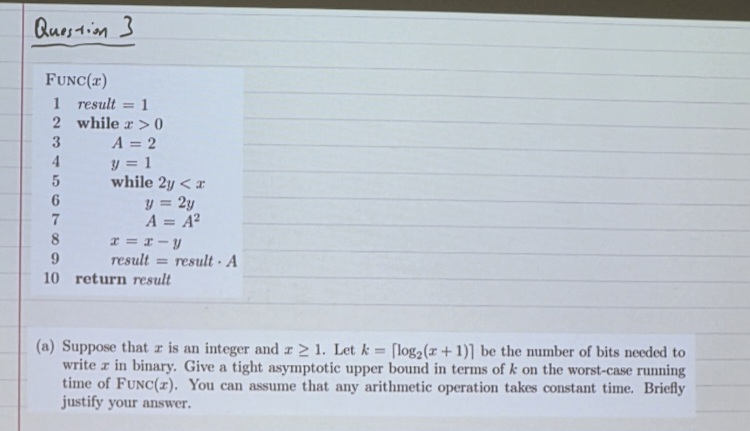
\includegraphics{csc265/figures/tut1q3.jpg}

\begin{problem}
Given an implementation for the predecessor operation on a binary search tree $T$, which gives a key $k$, return a pointer to a node $T$ with the largest key less than $k$. 
\end{problem}
